% Aberdeen style guide should be followed when using this
% layout. Their template powerpoint slide is used to extract the
% Aberdeen color and logo but is otherwise ignored (it has little or
% no formatting in it anyway).   
% 
% http://www.abdn.ac.uk/documents/style-guide.pdf

%%%%%%%%%%%%%%%%%%%% Document Class Settings %%%%%%%%%%%%%%%%%%%%%%%%%
% Pick if you want slides, or draft slides (no animations)
%%%%%%%%%%%%%%%%%%%%%%%%%%%%%%%%%%%%%%%%%%%%%%%%%%%%%%%%%%%%%%%%%%%%%%
%Normal document mode%
%\documentclass[10pt,compress,unknownkeysallowed]{beamer}
%Draft or handout mode 
\documentclass[10pt,compress,handout,unknownkeysallowed]{beamer}
%\documentclass[10pt,compress,handout,ignorenonframetext,unknownkeysallowed]{beamer}

%%%%%%%%%%%%%%%%%%%% General Document settings %%%%%%%%%%%%%%%%%%%%%%%
% These settings must be set for each presentation
%%%%%%%%%%%%%%%%%%%%%%%%%%%%%%%%%%%%%%%%%%%%%%%%%%%%%%%%%%%%%%%%%%%%%%
\newcommand{\shortname}{jefferson.gomes@abdn.ac.uk}
\newcommand{\fullname}{Dr Jeff Gomes}
\institute{School of Engineering}
\newcommand{\emailaddress}{}%jefferson.gomes@abdn.ac.uk}
\newcommand{\logoimage}{../../FigBanner/UoAHorizBanner}
\title{Chemical Thermodynamics (EX3029)}
\subtitle{Module 5: Chemical Reaction Equilibrium}
\date[ ]{ }



%%%%%%%%%%%%%%%%%%%%%%%%%%%%%%%%%%%%%%%%%%%%%%%%%%%%%%%%%%%%%%%%%%%%%%%%%%%%%%%
% BABEL and LANGUAGES %%%%%%%%%%%%%%%%%%%%%%%%%%%%%%%%%%%%%%%%%%%%%%%%%%%%%%%%%
%%%%%%%%%%%%%%%%%%%%%%%%%%%%%%%%%%%%%%%%%%%%%%%%%%%%%%%%%%%%%%%%%%%%%%%%%%%%%%%
% \usepackage{listings}                   % it is a source code printer for LATEX
                                          % \lstset{language=Python}
                                          % \lstinputlisting{source.py}   % command used to pretty-print stand alone files
\usepackage[english]{babel}               % [french, frenchb, english, ]
    % http://forum.mathematex.net/latex-f6/les-puces-avec-babel-t4256.html
    % http://www.grappa.univ-lille3.fr/FAQ-LaTeX/11.1.html


%%%%%%%%%%%%%%%%%%%%%%%%%%%%%%%%%%%%%%%%%%%%%%%%%%%%%%%%%%%%%%%%%%%%%%%%%%%%%%%
% FONTS and ENCODING %%%%%%%%%%%%%%%%%%%%%%%%%%%%%%%%%%%%%%%%%%%%%%%%%%%%%%%%%%
%%%%%%%%%%%%%%%%%%%%%%%%%%%%%%%%%%%%%%%%%%%%%%%%%%%%%%%%%%%%%%%%%%%%%%%%%%%%%%%
%
% See:
% http://tex.stackexchange.com/questions/59702/suggest-a-nice-font-family-for-my-basic-latex-template-text-and-math-i-am
%

\usepackage{lmodern}        % Latin Modern family of fonts. Very much like Computer Modern, but with many more glyphs 
                            % (e.g., for characters with accents, glyphs, cedillas, etc)
\usepackage[T1]{fontenc}    % fontenc is oriented to output, that is, what fonts to use for printing characters. 
                            % http://tex.stackexchange.com/questions/44694/fontenc-vs-inputenc 
                            % http://tex.stackexchange.com/questions/664/why-should-i-use-usepackaget1fontenc

% Change some fonts or the whole font family (i.e. serif, sans serif, monospace, and 'math')
    % \usepackage[varg, cmintegrals, cmbraces, ]{newtxtext,newtxmath}  % Other options: libertine, uprightGreek (U.S.) or slantedGreek (ISO), etc...
     \usepackage{tgtermes}                                            % Only serif ("TeX-Gyre" text)
    % \usepackage{kpfonts}                                             % "Kepler" fonts
    % \usepackage{mathpazo}                                            % Based on Hermann Zapf's Palatino font
    % \usepackage{txfonts}                                             % More than a decade old
    % \usepackage{pslatex}                                             % Obsolete?
    %  - \usepackage{mathptmx}
    %  - \usepackage[scaled=.90]{helvet}
    %  - \usepackage{courier}

% \usepackage{textcomp}     % required for special glyphs
% \usepackage{bm}           % load after all math to give access to bold math
\usepackage[utf8]{inputenc} % inputenc allows the user to input accented characters directly from the keyboard; 
                            % utf8x : much broader but less compatible ; latin1 : old?
                            % http://tex.stackexchange.com/questions/44694/fontenc-vs-inputenc

% See:
% http://tex.stackexchange.com/questions/59626/nicely-force-66-characters-per-line
%
% pslatex is a very obsolete package and that its descendant mathptmx is rather inadequate for serious typesetting involving math.
% If you don't need mathematics, other choices based on (Linotype) Times Roman are
%  - tgtermes
%  - newtxtext (based on txfonts, but with corrected metrics) (with its companion math package newtxmath)
%
%
% See:
% http://www.latex-community.org/forum/viewtopic.php?f=8&t=6637
%
% (times, helvet, courier)
% pslatex and txfonts produce (almost) same resutls.
% pslatex supposedly obsolete
% txfonts supposedly up-to-date
%
%
% See:
% ftp://ftp.rrzn.uni-hannover.de/pub/mirror/tex-archive/info/l2tabu/english/l2tabuen.pdf
% or 
% ftp://ftp.dante.de/tex-archive/info/l2tabu/english/l2tabuen.pdf
% in
% 2.3.3 pslatex.sty
%
% pslatex uses a Courier font scaled too narrowly.
% Its main disadvantage is that it does not work with T1 and TS1 encodings.
% So replace:
% \usepackage{pslatex} or \usepackage{txfonts}
% by all three:
% - \usepackage{mathptmx}
% - \usepackage[scaled=.90]{helvet}
% - \usepackage{courier}
%
%
% See:
% http://xpt.sourceforge.net/techdocs/language/latex/latex32-LaTeXAndFonts/single/
% or http://thirteen-01.stat.iastate.edu/wiki/LaTeXFonts
% or http://www.tex.ac.uk/tex-archive/info/beginlatex/html/chapter8.html
%
% When changing fonts, you can change all of the default fonts at once with the following commands:
% 
% Command     Changes the defaults to
% 
% times       Times, Helvetica, Courier
% pslatex     same as Times, but uses a specially narrowed Courier. This is preferred over Times because of the way it handles Courier.
% newcent     New Century Schoolbook, Avant Garde, Courier
% palatino    Palatino, Helevetica, Courier
% palatcm     changes the Roman to Palatino only, but uses CM mathematics
% kpfonts     "Kepler" fonts. A very nicely evolved set of fonts also based originally on Palatino, but with many special features.
%
%
% See:
% http://tex.stackexchange.com/questions/59702/suggest-a-nice-font-family-for-my-basic-latex-template-text-and-math-i-am
%
% There are, of course, many other font packages, most of which provide "only" text-mode fonts.
% Among these are the "TeX-Gyre" font families: 
%  - Termes (a Times Roman clone), 
%  - Pagella (a Palatino clone), and 
%  - Schola (a Century Schoolbook clone); 
% one would load the packages tgtermes, tgpagella, and tgschola, respectively, to access these fonts.
% However, as these are text fonts, you still need to choose a suitable math font.
% 
% Still another possibility you may want to look into is the Linux Libertine font family, to be loaded via the libertine-legacy package.
% If you like this text font and wish to employ the newtxmath package, be sure to load the newtxmath package with the libertine option set;
% doing so will set up a special set of math-mode fonts that harmonizes well with the libertine text fonts.
% 
%
% See also:
% http://tex.stackexchange.com/questions/56876/times-new-roman-fonts-and-maths-without-mathptmx
%
%
% For a comparison, in:
% /home/christophe/Personal/Truc_Et_Astuce_Informatik/LaTeX/comparison_font_types/,
% see: 
% computer.pdf  lmodern.pdf  pslatex.pdf  test_font_type.pdf  three_replacements.pdf  txfonts.pdf
%


%%%%%%%%%%%%%%%%%%%%%%%%%%%%%%%%%%%%%%%%%%%%%%%%%%%%%%%%%%%%%%%%%%%%%%%%%%%%%%%
% AMS MATH %%%%%%%%%%%%%%%%%%%%%%%%%%%%%%%%%%%%%%%%%%%%%%%%%%%%%%%%%%%%%%%%%%%%
%%%%%%%%%%%%%%%%%%%%%%%%%%%%%%%%%%%%%%%%%%%%%%%%%%%%%%%%%%%%%%%%%%%%%%%%%%%%%%%
% \usepackage{amsmath}      % loads amstext, amsbsy, amsopn but not amssymb
                            % equation stuff (eqref, subequations, equation, align, gather, flalign, multline, alignat, split...)
% \usepackage{amsfonts}     % may be redundant with amsmath
% \usepackage{amssymb}      % may be redundant with amsmath
% \numberwithin{equation}{section}  % reset equation counters at start of each "section" and prefix numbers by section number
% \numberwithin{figure}{section}    % reset figure   counters at start of each "section" and prefix numbers by section number


%%%%%%%%%%%%%%%%%%%%%%%%%%%%%%%%%%%%%%%%%%%%%%%%%%%%%%%%%%%%%%%%%%%%%%%%%%%%%%%
% LAY OUT %%%%%%%%%%%%%%%%%%%%%%%%%%%%%%%%%%%%%%%%%%%%%%%%%%%%%%%%%%%%%%%%%%%%%
%%%%%%%%%%%%%%%%%%%%%%%%%%%%%%%%%%%%%%%%%%%%%%%%%%%%%%%%%%%%%%%%%%%%%%%%%%%%%%%
%
% See:
% http://tex.stackexchange.com/questions/59626/nicely-force-66-characters-per-line
% (must be after pslatex, tgterms, etc...)
%
% a) (but works mostly for a4paper, and changes top and bottom margin too...)
% \usepackage[DIV=calc]{typearea}
%
% or
%
% b) (but you have to choose the value and the margin ratio depending on the class...)
% \newlength{\alphabet}
% \settowidth{\alphabet}{\normalfont abcdefghijklmnopqrstuvwxyz}
% \usepackage{geometry}
% \geometry{%
% textwidth=2.5\alphabet,% (Note: 2.5 * 26 = 65)
% hmarginratio={2:3}}    % (Problem: geometry uses 2:3 as default for twoside and 1:1 for oneside,
%                        % independently of what the class thinks about the margins)

% \usepackage{layout}       % use \layout in the tex file to see the values
% \usepackage{layouts}      % it extends the functionality of layout, allowing you to do much, much more
                            % some commands: \pagelayout, \pagevalues, \pagedesign, ...
% \usepackage[cm]{fullpage} % set 'default' full page
% \usepackage{geometry}     % very customizable margins. Under some (rare) circumstances, should be loaded after hyperref
% \usepackage{anysize}      % \marginsize{left}{right}{top}{bottom}
% \usepackage{pdflscape}    % include landscape layout pages (automatically rotate pages in pdf file for easier reading)
% \usepackage{multicol}     % for multi column environment
\usepackage{lipsum}         % to fill in with arbitrary text
\widowpenalty = 4000        % help suppress widows,  default = 4,000 (?), from 0 to 10 000 (from 300 to 1 000 recommended, 10 000 not recommended)
\clubpenalty  = 4000        % help suppress orphans, default = 4,000 (?), from 0 to 10 000 (from 300 to 1 000 recommended, 10 000 not recommended)
\usepackage[final, babel]{microtype} % many good lay-out/justification effects, see:
                                     % texblog.net/latex-archive/layout/pdflatex-microtype/


%%%%%%%%%%%%%%%%%%%%%%%%%%%%%%%%%%%%%%%%%%%%%%%%%%%%%%%%%%%%%%%%%%%%%%%%%%%%%%%
% EMBED FILEs %%%%%%%%%%%%%%%%%%%%%%%%%%%%%%%%%%%%%%%%%%%%%%%%%%%%%%%%%%%%%%%%%
%%%%%%%%%%%%%%%%%%%%%%%%%%%%%%%%%%%%%%%%%%%%%%%%%%%%%%%%%%%%%%%%%%%%%%%%%%%%%%%
\usepackage{embedfile}    % embed (attach) any files (eg tex source) to a PDF document.
                          % Currently only supported driver is pdfTEX >= 1.30 in PDF mode
%\embedfile{to_post.tex}


%%%%%%%%%%%%%%%%%%%%%%%%%%%%%%%%%%%%%%%%%%%%%%%%%%%%%%%%%%%%%%%%%%%%%%%%%%%%%%%
% EASY EDITS %%%%%%%%%%%%%%%%%%%%%%%%%%%%%%%%%%%%%%%%%%%%%%%%%%%%%%%%%%%%%%%%%%
%%%%%%%%%%%%%%%%%%%%%%%%%%%%%%%%%%%%%%%%%%%%%%%%%%%%%%%%%%%%%%%%%%%%%%%%%%%%%%%
\usepackage{ifdraft}        % ask for selective behavior depending on the draft option (used for waterdraftmark, not draftmark)
% \usepackage{comment}      % provide new {comment} environment: all text inside the environment is ignored.
% \usepackage{fixme}        % allow nice comment / warning system, displayed in draft mode in right margin ; % [status=draft]
% \usepackage{lineno}       % number all lines in left margin if activated with \linenumbers
% \linenumbers


%%%%%%%%%%%%%%%%%%%%%%%%%%%%%%%%%%%%%%%%%%%%%%%%%%%%%%%%%%%%%%%%%%%%%%%%%%%%%%%
% GRAPHICX %%%%%%%%%%%%%%%%%%%%%%%%%%%%%%%%%%%%%%%%%%%%%%%%%%%%%%%%%%%%%%%%%%%%
%%%%%%%%%%%%%%%%%%%%%%%%%%%%%%%%%%%%%%%%%%%%%%%%%%%%%%%%%%%%%%%%%%%%%%%%%%%%%%%
% \usepackage[final]{graphicx} % options = [final]  = all graphics displayed, regardless of draft option in class
                               % options = [pdftex] = necessary (?) if import PDF files
                               % no option : when importing ps- and eps-files (?)
% \graphicspath{{../images/}}  % tell LaTeX where to look for images
% \DeclareGraphicsExtensions{.pdf, .PDF, .jpg, .JPG, .jpeg, .JPEG, .png, .PNG, .bmp, .BMP, .eps, .ps}
\usepackage{float}                      % Improved interface for floating objects ; add [H] option


%%%%%%%%%%%%%%%%%%%%%%%%%%%%%%%%%%%%%%%%%%%%%%%%%%%%%%%%%%%%%%%%%%%%%%%%%%%%%%%
% FILIGREE %%%%%%%%%%%%%%%%%%%%%%%%%%%%%%%%%%%%%%%%%%%%%%%%%%%%%%%%%%%%%%%%%%%%
%%%%%%%%%%%%%%%%%%%%%%%%%%%%%%%%%%%%%%%%%%%%%%%%%%%%%%%%%%%%%%%%%%%%%%%%%%%%%%%
% draftmark : newer and better package but not on Phil's computers,
% in particular, draftmark has a "ifdraft" option included...
%
\ifdraft{
\usepackage{draftwatermark} % add watermark ("draft", "confidential"...)
                            % option: [firstpage] (insert on only the first page)
\SetWatermarkText{COPY~---~DRAFT}
\SetWatermarkAngle{55}
\SetWatermarkScale{6.0}
\SetWatermarkLightness{0.85}
\SetWatermarkFontSize{12 pt}
}{}


\renewcommand{\insertframenumber}{\theframenumber}
\renewcommand{\theframenumber}{\thesection-\arabic{framenumber}}
\renewcommand{\thesubsectionslide}{\thesection-\arabic{framenumber}}
\setbeamertemplate{headline}[text line]{This is frame: \insertframenumber}
\AtBeginSection{\setcounter{framenumber}{0}}


%%%%%%%%%%%%%%%%%%%% Template settings %%%%%%%%%%%%%%%%%%%%%%%%%%%%%%%
% You shouldn't have to change below this line, unless you want to.
%%%%%%%%%%%%%%%%%%%%%%%%%%%%%%%%%%%%%%%%%%%%%%%%%%%%%%%%%%%%%%%%%%%%%%
\usecolortheme{whale}
\useoutertheme{infolines}

% Use the fading effect for items that are covered on the current
% slide.
\beamertemplatetransparentcovered

% We abuse the author command to place all of the slide information on
% the title page.
\author[\shortname]{%
  \fullname\\\ttfamily{\emailaddress}
}


%At the start of every section, put a slide indicating the contents of the current section.
\AtBeginSection[] {
  \begin{frame}
    \frametitle{Section Outline}
    \tableofcontents[currentsection]
  \end{frame}
}

% Allow the inclusion of movies into the Presentation! At present,
% only the Okular program is capable of playing the movies *IN* the
% presentation.
\usepackage{multimedia}
\usepackage{animate}

%% Handsout -- comment out the lines below to create handstout with 4 slides in a page with space for comments
\usepackage{handoutWithNotes}

\mode<handout>
{
\usepackage{pgf,pgfpages}

\pgfpagesdeclarelayout{2 on 1 boxed with notes}
{
\edef\pgfpageoptionheight{\the\paperheight} 
\edef\pgfpageoptionwidth{\the\paperwidth}
\edef\pgfpageoptionborder{0pt}
}
{
\setkeys{pgfpagesuselayoutoption}{landscape}
\pgfpagesphysicalpageoptions
    {%
        logical pages=4,%
        physical height=\pgfpageoptionheight,%
        physical width=\pgfpageoptionwidth,%
        last logical shipout=2%
    } 
\pgfpageslogicalpageoptions{1}
    {%
    border code=\pgfsetlinewidth{1pt}\pgfstroke,%
    scale=1,
    center=\pgfpoint{.25\pgfphysicalwidth}{.75\pgfphysicalheight}%
    }%
\pgfpageslogicalpageoptions{2}
    {%
    border code=\pgfsetlinewidth{1pt}\pgfstroke,%
    scale=1,
    center=\pgfpoint{.25\pgfphysicalwidth}{.25\pgfphysicalheight}%
    }%
\pgfpageslogicalpageoptions{3}
    {%
    border shrink=\pgfpageoptionborder,%
    resized width=.7\pgfphysicalwidth,%
    resized height=.5\pgfphysicalheight,%
    center=\pgfpoint{.75\pgfphysicalwidth}{.29\pgfphysicalheight},%
    copy from=3
    }%
\pgfpageslogicalpageoptions{4}
    {%
    border shrink=\pgfpageoptionborder,%
    resized width=.7\pgfphysicalwidth,%
    resized height=.5\pgfphysicalheight,%
    center=\pgfpoint{.75\pgfphysicalwidth}{.79\pgfphysicalheight},%
    copy from=4
    }%

\AtBeginDocument
    {
    \newbox\notesbox
    \setbox\notesbox=\vbox
        {
            \hsize=\paperwidth
            \vskip-1in\hskip-1in\vbox
            {
                \vskip1cm
                Notes\vskip1cm
                        \hrule width\paperwidth\vskip1cm
                    \hrule width\paperwidth\vskip1cm
                        \hrule width\paperwidth\vskip1cm
                    \hrule width\paperwidth\vskip1cm
                        \hrule width\paperwidth\vskip1cm
                    \hrule width\paperwidth\vskip1cm
                    \hrule width\paperwidth\vskip1cm
                    \hrule width\paperwidth\vskip1cm
                        \hrule width\paperwidth
            }
        }
        \pgfpagesshipoutlogicalpage{3}\copy\notesbox
        \pgfpagesshipoutlogicalpage{4}\copy\notesbox
    }
}
}

%\pgfpagesuselayout{2 on 1 boxed with notes}[letterpaper,border shrink=5mm]
%\pgfpagesuselayout{2 on 1 boxed with notes}[letterpaper,border shrink=5mm]


%%%%%%%%%% Chemical Reactions %%%%%%%%%%%%%%%%

\usepackage[T1]{fontenc}
\usepackage[utf8]{inputenc}
\usepackage{lmodern}
\usepackage[version=3]{mhchem}
\makeatletter
\newcounter{reaction}
%%% >> for article <<
%\renewcommand\thereaction{C\,\arabic{reaction}}
%%% << for article <<
%%% >> for report and book >>
%\renewcommand\thereaction{C\,\thechapter.\arabic{reaction}}
%\@addtoreset{reaction}{chapter}
%%% << for report and book <<
\newcommand\reactiontag{\refstepcounter{reaction}\tag{\thereaction}}
\newcommand\reaction@[2][]{\begin{equation}\ce{#2}%
\ifx\@empty#1\@empty\else\label{#1}\fi%
\reactiontag\end{equation}}
\newcommand\reaction@nonumber[1]{\begin{equation*}\ce{#1}%
\end{equation*}}
\newcommand\reaction{\@ifstar{\reaction@nonumber}{\reaction@}}
\makeatother

%%%%%%%%%%%%%%%%%%%%%%%%%%%%%%%%%%%%%%%%%%%%%%


%%%%% Color settings
\usepackage{color}
%% The background color for code listings (i.e. example programs)
\definecolor{lbcolor}{rgb}{0.9,0.9,0.9}%
\definecolor{UoARed}{rgb}{0.64706, 0.0, 0.12941}
\definecolor{UoALight}{rgb}{0.85, 0.85, 0.85}
\definecolor{UoALighter}{rgb}{0.92, 0.92, 0.92}
\setbeamercolor{structure}{fg=UoARed} % General background and higlight color
\setbeamercolor{frametitle}{bg=black} % General color
\setbeamercolor{frametitle right}{bg=black} % General color
\setbeamercolor{block body}{bg=UoALighter} % For blocks
\setbeamercolor{structure}{bg=UoALight} % For blocks
% Rounded boxes for blocks
\setbeamertemplate{blocks}[rounded]

%%%%% Font settings
% Aberdeen requires the use of Arial in slides. We can use the
% Helvetica font as its widely available like so
% \usepackage{helvet}
% \renewcommand{\familydefault}{\sfdefault}
% But beamer already uses a sans font, so we will stick with that.

% The size of the font used for the code listings.
\newcommand{\goodsize}{\fontsize{6}{7}\selectfont}

% Extra math packages, symbols and colors. If you're using Latex you
% must be using it for formatting the math!
\usepackage{amscd,amssymb} \usepackage{amsfonts}
\usepackage[mathscr]{eucal} \usepackage{mathrsfs}
\usepackage{latexsym} \usepackage{amsmath} \usepackage{bm}
\usepackage{amsthm} \usepackage{textcomp} \usepackage{eurosym}
% This package provides \cancel{a} and \cancelto{a}{b} to "cancel"
% expressions in math.
\usepackage{cancel}

\usepackage{comment} 

% Get rid of font warnings as modern LaTaX installations have scalable
% fonts
\usepackage{type1cm} 

%\usepackage{enumitem} % continuous numbering throughout enumerate commands

% For exact placement of images/text on the cover page
\usepackage[absolute]{textpos}
\setlength{\TPHorizModule}{1mm}%sets the textpos unit
\setlength{\TPVertModule}{\TPHorizModule} 

% Source code formatting package
\usepackage{listings}%
\lstset{ backgroundcolor=\color{lbcolor}, tabsize=4,
  numberstyle=\tiny, rulecolor=, language=C++, basicstyle=\goodsize,
  upquote=true, aboveskip={1.5\baselineskip}, columns=fixed,
  showstringspaces=false, extendedchars=true, breaklines=false,
  prebreak = \raisebox{0ex}[0ex][0ex]{\ensuremath{\hookleftarrow}},
  frame=single, showtabs=false, showspaces=false,
  showstringspaces=false, identifierstyle=\ttfamily,
  keywordstyle=\color[rgb]{0,0,1},
  commentstyle=\color[rgb]{0.133,0.545,0.133},
  stringstyle=\color[rgb]{0.627,0.126,0.941}}

% Allows the inclusion of other PDF's into the final PDF. Great for
% attaching tutorial sheets etc.
\usepackage{pdfpages}
\setbeamercolor{background canvas}{bg=}  

% Remove foot note horizontal rules, they occupy too much space on the slide
\renewcommand{\footnoterule}{}

% Force the driver to fix the colors on PDF's which include mixed
% colorspaces and transparency.
\pdfpageattr {/Group << /S /Transparency /I true /CS /DeviceRGB>>}

% Include a graphics, reserve space for it but
% show it on the next frame.
% Parameters:
% #1 Which slide you want it on
% #2 Previous slides
% #3 Options to \includegraphics (optional)
% #4 Name of graphic
\newcommand{\reserveandshow}[4]{%
\phantom{\includegraphics<#2|handout:0>[#3]{#4}}%
\includegraphics<#1>[#3]{#4}%
}

\newcommand{\frc}{\displaystyle\frac}
\newcommand{\red}{\textcolor{red}}
\newcommand{\blue}{\textcolor{blue}}
\newcommand{\green}{\textcolor{green}}
\newcommand{\purple}{\textcolor{purple}}
\newcommand{\eg}{{\it e.g., }}
\newcommand{\ie}{{\it i.e., }}
\newcommand{\wrt}{{\it wrt }}
\newcommand{\Partial}[3][error]{\left(\frc{\partial #1}{\partial #2}\right)_{#3}}
\newcommand{\mfr}[3][error]{#1_{#2}^{\left(#3\right)}} 
\newcommand{\summation}[3][error]{\sum\limits_{#2}^{#3}#1}


 
\begin{document}

% Title page layout
\begin{frame}
  \titlepage
  \vfill%
  \begin{center}
    \includegraphics[clip,width=0.8\textwidth]{\logoimage}
  \end{center}
\end{frame}

% Table of contents
\frame{ \frametitle{Slides Outline}
  \tableofcontents
}


%%%%%%%%%%%%%%%%%%%% The Presentation Proper %%%%%%%%%%%%%%%%%%%%%%%%%
% Fill below this line with \begin{frame} commands! It's best to
% always add the fragile option incase you're going to use the
% verbatim environment.
%%%%%%%%%%%%%%%%%%%%%%%%%%%%%%%%%%%%%%%%%%%%%%%%%%%%%%%%%%%%%%%%%%%%%%

%%%
%%% SECTION
%%%
\section{Learning Objectives}

%%%
%%% Slides
%%%
\begin{frame}
 \frametitle{Learning Objectives}
   \begin{enumerate}
     \item Select appropriate molar stoichiometric coefficients to balance chemical reactions and to determine reaction coordinates;
     \item Identify if a chemical reaction is either exothermic or endothermic;
     \item Assess the heat associated with any chemical reaction;
     \item Calculate the equilibrium constant at any reaction condition;
     \item Understand the influences of pressure, stoichiometric feed and inerts on reaction equilibrium.
   \end{enumerate}
\end{frame}

%%%
%%% Slides
%%%
\begin{frame}
 \frametitle{Aims and Objectives}
   \begin{enumerate}
     \item<1-> In the previous modules we studied thermodynamic relations in non-reactive systems;
     \item<1-> In Modules 3 and 4 we focused on systems involving components in gas and liquid phases behaving as ideal and non-ideal mixtures;
     \item<2-> Most of the thermodynamic relations can be extended to systems involving single and multiple reactions across single and multiple phases;
     \item<2-> The aim of this module is {\bf to study equilibrium state of homogeneous (\ie single phase) chemical reactions.}
   \end{enumerate}
\end{frame}


%%%
%%% SECTION
%%%
\section{Bibliography}
\begin{frame}
 \frametitle{Suggested References}
  Literature relevant for this module:
  \begin{enumerate}[(i)]
     \item\label{SVN_Book} J.M. Smith, H.C. Van Ness, M.M. Abbott, $\lq$Introduction to Chemical Engineering Thermodynamics', 6$^{th}$ Edition: Chapter 13;
     \item\label{Sandle_Book} S.I. Sandler, $\lq$Chemical, Biochemical and Engineering Thermodynamics', 4$^{th}$ Edition: Chapters 8.3-5 and 13;
     \item\label{Lue_Book} L. Lue, $\lq$Chemical Thermodynmics', {\it eBook at bookboon.com}, Chapter 12;
     \item\label{Balmer_Book}R.T. Balmer, $\lq$Modern Engineering Thermodynamics', Chapter 15;
     \item\label{Moran_Book} M.J. Moran and H.N. Shapiro, $\lq$Fundamentals of Engineering Thermodynamics', 5$^{\text{th}}$ Edition, Chapter 14;
     \item\label{Devoe_Book} H. Devoe, $\lq$Thermodynamics and Chemistry', 2$^{\text{nd}}$ Edition, Chapter 11;
     \item\label{Atkins_Book} P. Atkins and J. de Paula, $\lq$Physical Chemistry', 8$^{\text{th}}$ Edition: Chapters 2 and 5.
  \end{enumerate}
\end{frame}


%%%
%%% SECTION
%%%
\section{Introduction}

%%%
%%% Slide
%%%
%\scriptsize
\begin{frame}
  \frametitle{Chemical Reaction Process}
      Given the chemical reaction in gas phase:

          \vspace{-.0cm}
          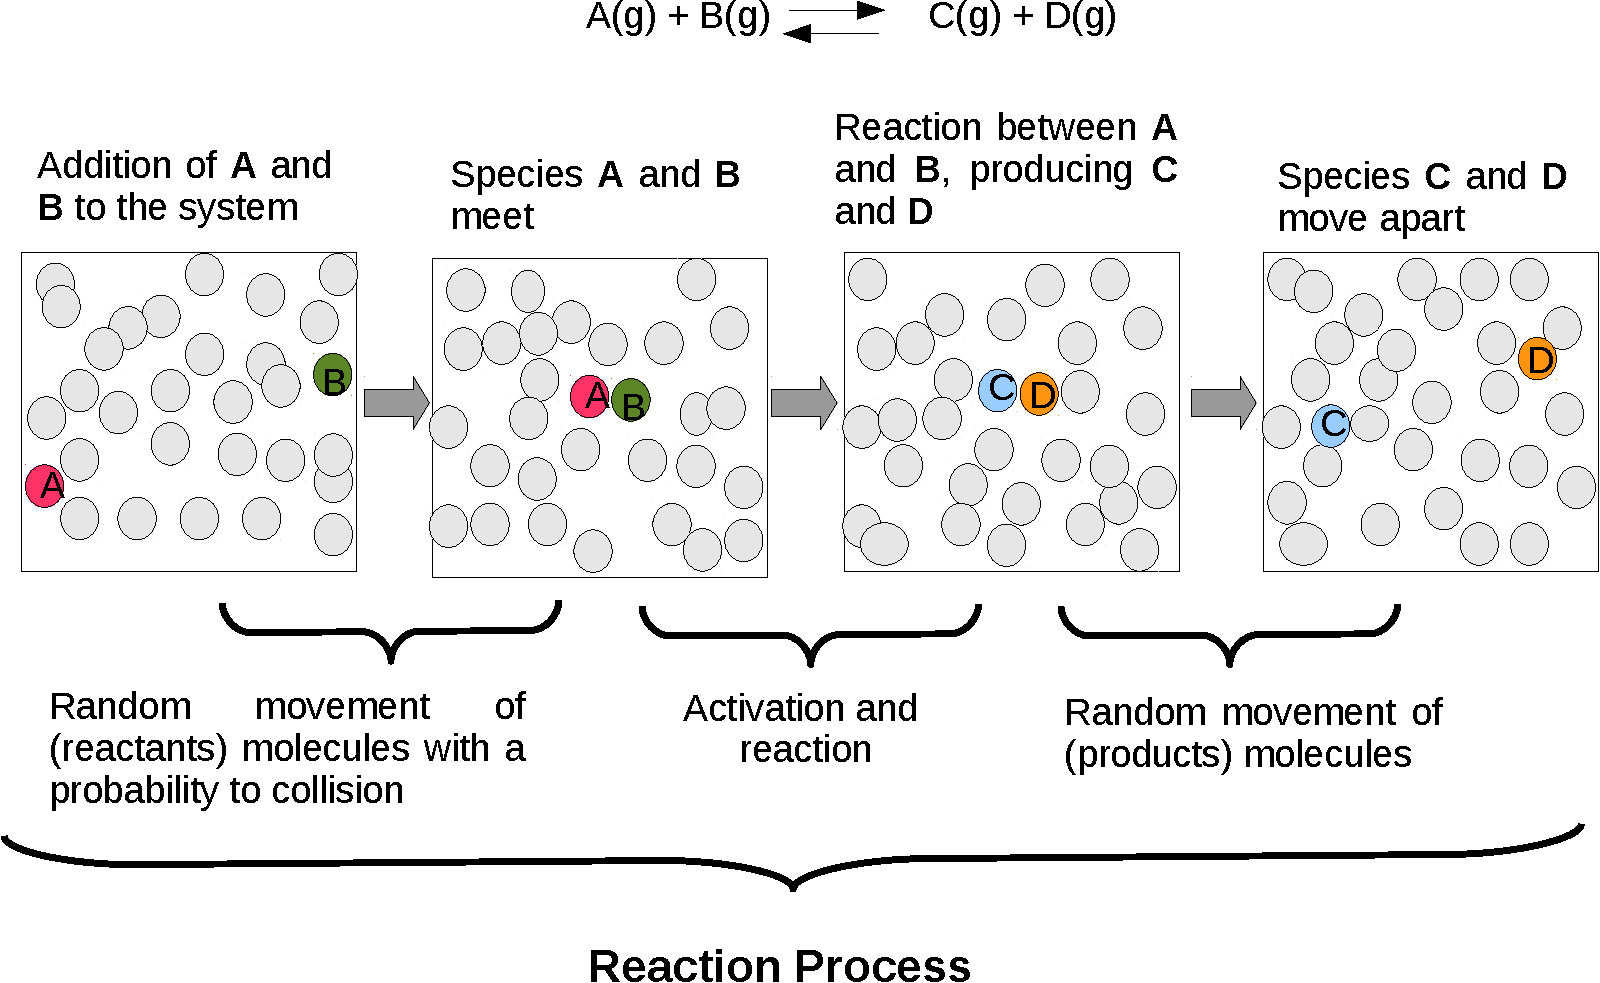
\includegraphics[width=.95\columnwidth,clip]{./../Pics/ChemicalReactionsDiagram2}
\end{frame}
\normalsize


%%%
%%% Slide
%%%
%\scriptsize
\begin{frame}
  \frametitle{Chemical Reaction Process: \blue{Diffusion} $\times$ Kinetics $\times$ Thermodynamics}

  \begin{block}{\begin{center}General Chemical Reaction\end{center}}
     Given the chemical reaction below
        \reaction{ A (g) + B(g) <=>[r_{k}] C (g) + D (g) }
  \end{block}  

   \begin{enumerate}[a)]
       \item<1-> The process for molecules to travel across the 'pool' of molecules is called \blue{diffusion};
       \item<2-> In general the reacting chemical species molecules can be in gas, liquid and/or solid phases and;
       \item<2-> {\it Molecular diffusion} may occur in \underline{any} of these phases;
       \item<3-> \blue{Diffusivity} (\ie rate of diffusion) has an order \wrt the reaction phase:
               \begin{center} gas > liquid > solid\end{center}
       \item<3-> \blue{Molecular diffusion} processes are mathematically described by the \red{Fick's law}
   \end{enumerate}
\end{frame}
\normalsize


%%%
%%% Slide
%%%
%\scriptsize
\begin{frame}
  \frametitle{Chemical Reaction Process: Diffusion $\times$ \blue{Kinetics} $\times$ Thermodynamics}

  \begin{block}{\begin{center}General Chemical Reaction\end{center}}
     Given the chemical reaction below
        \reaction{ A (g) + B(g) <=>[r_{k}] C (g) + D (g) }
  \end{block}  

   \begin{enumerate}[a)]
       \item<1-> \red{$r_{k}$} represents the \blue{rate of reaction}, \ie the `speed' of the reaction. The \blue{rate of reaction} measures how 'fast' or 'slow' reactants ($A$ and $B$) has been consumed and products ($C$ and $D$) have been produced;
       \item<1-> Therefore, the \blue{rate of reaction is proportional to the amount of chemical species} in the system, \eg
             \begin{displaymath}
                  r_{k} = \kappa [A]^{m_{1}}[B]^{m_{2}}[C]^{m_{3}}[D]^{m_{4}},
             \end{displaymath}
             where the proportionality constant $\kappa$ is the \red{\it rate of reaction constant}, [$\Theta$] is the concentration of the chemical species and coefficients $m_{i}$ are the order of the reactant;
       \item<1-> \blue{Chemical kinetics studies \underline{reactions' progress}}, \ie `speed' of consumption of reactants and production of products and \red{mechanisms of reactions};
   \end{enumerate}
\end{frame}
\normalsize

%%%
%%% Slide
%%%
%\scriptsize
\begin{frame}
  \frametitle{Chemical Reaction Process: \blue{Diffusion} $\times$ \blue{Kinetics} $\times$ Thermodynamics}


   \begin{enumerate}[a)]
       \item<1-> \blue{Molecular diffusion} and \blue{chemical kinetics} are different mechanisms in chemical reactions;
       \item<2-> Whereas the former determines the {\it 'degree of spreading'} of species in the reaction media (\ie gas, liquid and/or solid phases) and the probability of molecular collisions;
       \item<3-> The later determines how species (\ie molecules, atoms, ions, functional groups) will dissociate and combine to form new species and, most of all;
        \item<4-> How fast these processes (dissociation and combination, \ie reactions) will take place.
   \end{enumerate}
\end{frame}
\normalsize


%%%
%%% Slide
%%%
%\scriptsize
\begin{frame}
  \frametitle{Chemical Reaction Process: Diffusion $\times$ Kinetics $\times$ \blue{Thermodynamics}}

  \begin{block}{\begin{center}General Chemical Reaction\end{center}}
     %Given the chemical reaction below
        \reaction{ A (g) + B (g) <=>[K_{e}] C (g) + D (g) }
  \end{block}  
   \begin{enumerate}[a)]
       \item<1-> \red{$K_{e}$} is the \red{thermodynamic equilibrium constant} and `measures how much product and reactants exist in the mixture at equilibrium',
       \item<1-> The equilibrium constant takes into account the conditions ($T$ and $P$) that lead a given set of reactions into equilibrium, \eg
             \begin{displaymath}
                  K_{e} = \frc{a_{C}a_{D}}{a_{A}a_{B}}
             \end{displaymath}
             where $a_{i}$ is \blue{activity of chemical species}. 
       \item<1-> \blue{Chemical Reaction Thermodynamics } studies state functions and conditions necessary to {\it maximum} conversion of species;
       \item<1-> Reactions that leads to $\sim$100$\%$ of conversion are called \blue{irreversible}, whereas;
       \item<1-> Reactions that have conversion rates significantly smaller than 100$\%$ are called \blue{reversible}.
   \end{enumerate}
\end{frame}
\normalsize

%%%
%%% Slide
%%%
%\scriptsize
\begin{frame}
  \frametitle{Homogeneous $\times$ Heterogeneous Chemical Reactions}
  \visible<1->{\begin{block}{\begin{center}Homogeneous Chemical Reaction\end{center}}
        \reaction[chemreaction:reaction0c]{ A (g) <=> B (g) + C (g) }
        Reactions that occur in a single phase (either gaseous, liquid or solid) are called \blue{homogeneous} reactions.
  \end{block} } 

  \visible<1->{\begin{block}{\begin{center}Heterogeneous Chemical Reaction\end{center}}
        \reaction[chemreaction:reaction0c]{ A (g) <=> B (s) + C (g) }
        Reactions that occur in multiple phases are called \blue{heterogeneous} reactions.
  \end{block}  }
\end{frame}
\normalsize


%%%
%%% SECTION
%%%
\section{Chemical Reactions}

%%%
%%% SUBSECTION
%%%
\subsection{Reaction Coordinate}

%%%
%%% Slide
%%%
%\scriptsize
\begin{frame}
  \frametitle{Reaction Coordinate}
  \begin{block}{\begin{center}General Chemical Reaction\end{center}}
        \reaction[chemreaction:reaction]{\nu_{1} A_{1} + \nu_{2} A_{2}  + ... \nu_{k} A_{k} <=>[\text{K$_{e}$}] \nu_{l} A_{l} + \nu_{m} A_{m} + ... + \nu_{z} A_{z} }
        where \red{$\nu_{i}$} represent \blue{molar stoichiometric coefficients} and $A_{i}$ are chemical species.
  \end{block}

  \begin{enumerate}[a)]
      \item<1-> The Standard notation \\
         \begin{center} 
            \begin{tabular}{l l}
           %\hline 
              {\it Reactants:} \red{negative $\nu_{i}$};  & \it{Product:} \blue{positive $\nu_{i}$},\\
           %\hline
            \end{tabular}
         \end{center}
         
       \item<2-> is adopted to enable writing chemical reactions in mathematical form:
         \begin{displaymath}
            \nu_{l} A_{l} + \nu_{m} A_{m} + \cdots + \nu_{z} A_{z} - \left( \nu_{1} A_{1} + \nu_{2} A_{2}  + \cdots \nu_{k} A_{k}\right) = 0;
         \end{displaymath}
  \end{enumerate}
\end{frame}
\normalsize




%%%
%%% Slide
%%%
%\scriptsize
\begin{frame}
  \frametitle{Reaction Coordinate}
  
  \begin{enumerate}\setcounter{enumi}{2}
     \item<1-> Change in quantities as reaction progresses:
        \visible<1->{\begin{displaymath}
           \frc{d n_{1}}{\nu_{1}}  =  \frc{d n_{2}}{\nu_{2}} = \cdots =  \frc{d n_{k}}{\nu_{k}} = \cdots = \frc{d n_{z}}{\nu_{z}}  \blue{\Longrightarrow \frc{d n_{i}}{\nu_{i}} = \text{constant} }
        \end{displaymath}}
    \item<2-> \red{Reaction coordinate $\varepsilon$},
        \visible<2->{\begin{displaymath}
           \frc{d n_{i}}{\nu_{i}} =  d \varepsilon_{i} \hspace{.5cm}\Longleftrightarrow\hspace{.5cm} d n_{i} = \nu_{i} d\varepsilon 
        \end{displaymath}}
    \item<3-> Mole fractions of species:
        \visible<3->{\begin{displaymath}
           y_{i} = \frc{n_{i}}{n} = \frc{n_{i,0}+\nu_{i}\varepsilon}{n_{0}+\nu\varepsilon}
        \end{displaymath}}     
  \end{enumerate}
\end{frame}
\normalsize




%%%
%%% Slide
%%%
%\scriptsize
\begin{frame}
  \frametitle{Reaction Coordinate for Multi-Reaction Systems}
  \begin{block}{\begin{center}General Chemical Reaction\end{center}}
        Given the reaction in multiple steps:
        \begin{displaymath}
           \visible<1->{\nu_{a}A(g) + \nu_{b}B(g) \Longleftrightarrow \nu_{c}C(g) + \nu_{d}D(g)}\visible<2->{ \begin{cases}
               \nu_{a,1}A(g) \longleftrightarrow \nu_{c,1}C(g) + \nu_{e,1}E(g) & \\
               \nu_{e,2}E(g) + \nu_{b,2}B(g) \longleftrightarrow \nu_{f,2}F(g) & \\
               \nu_{a,3}A(g) + \nu_{f,3}F(g) \longleftrightarrow \nu_{d,3}D(g) & 
           \end{cases}}
         \end{displaymath} 
         where \blue{$\nu_{i,j}$} is the stoichiometric coefficient of chemical species \blue{$i$} in reaction \blue{$j$}.
  \end{block}
        \begin{enumerate} \setcounter{enumi}{3}
           \item<3-> Multireaction progress:
               \visible<1->{\begin{displaymath}
                  d n_{i} = \sum\limits_{i}\nu_{i,j}d\varepsilon_{j}
               \end{displaymath}}
           \item<4-> Mole fractions of species:     
               \visible<2->{\begin{displaymath}
                  y_{i} = \frc{n_{i,0} + \sum\limits_{j}\nu_{i,j}\varepsilon_{j}} {n_{0} + \sum\limits_{j} \nu_{j}\varepsilon_{j}}
               \end{displaymath}}  
        \end{enumerate}
             \blue{where $j$ is the reaction index.}
\end{frame}
\normalsize


%%%
%%% SUBSECTION
%%%
\subsection{Standard Gibbs Free Energy of Reaction}


%%%
%%% Slide
%%%
%\scriptsize
\begin{frame}
  \frametitle{Formation Reaction}  
            \visible<1->{\begin{block}{\begin{center}Definition (Devoe, 2012)\end{center}} 
              ``The \red{formation reaction} of a substance is the reaction in which the substance, at a given temperature and in a given physical state, is \blue{formed from the constituent elements in their reference states at the same temperature}. ''
            \end{block}}
            
            \visible<2->{\begin{block}{\begin{center}Definition (Devoe, 2012)\end{center}} 
              ``The \red{reference state} of an element is usually chosen to be the \blue{standard state} of the element in the allotropic form and physical state that is stable at the given temperature and the standard pressure.''
            \end{block}}
\end{frame}
\normalsize


%%%
%%% Slide
%%%
%\scriptsize
\begin{frame}
  \frametitle{Standard Enthalpy of Formation}      
      \begin{enumerate}[a)]
         \item<1-> Let's consider the {\it exothermic} reaction to produce \red{CO$_{2}$} from \red{C} and \red{O$_{2}$},
            \begin{displaymath}
               C \left(\text{s}, \text{graphite}, P^{\circ}\right) + O_{2} \left(\text{g}, P^{\circ}\right) \Longleftrightarrow CO_{2} \left(\text{g}, P^{\circ}\right),
            \end{displaymath}
            \visible<2->{Product $\left(\text{CO}_{2}\right)$ is formed from the reaction of \blue{elemental reactants}, \ie \blue{atom} (\red{C}) and \blue{diatomic molecules} $\left(\red{\text{O}_{2}}\right)$. The reaction produces 393.52 kJ.mol$^{-1}$ of heat;}
            \visible<3->{\begin{block}{\begin{center}Definition (Devoe, 2012)\end{center}} 
              ``The \blue{standard molar enthalpy of formation} (or {\it standard molar heat of formation}) $\Delta H_{f}^{\circ}$, of a substance is the molar enthalpy change of substance produced in the \blue{formation reaction} of the substance in its standard state. The \blue{standard state} (or \blue{reference state} of a substance is its most stable state at the specified temperature and 1 atm.''
            \end{block}}
         \item<4-> By definition, $\Delta H_{f}^{\circ}$ for the \blue{reference state} of an \blue{element} $\left(\text{\eg C, O}_{2}, \text{Br}_{2}, \text{etc}\right)$ is \red{zero};
         \item<5-> Values of \red{standard molar enthalpy of formation} are tabulated for a number of chemical species.
      \end{enumerate}
\end{frame}
\normalsize



%%%
%%% Slide
%%%
%\scriptsize
\begin{frame}
  \frametitle{$\Delta H_{f}^{\circ}$ and $\Delta G_{f}^{\circ}$ (Moran $\&$ Shapiro, 2006)}
     \begin{center}
       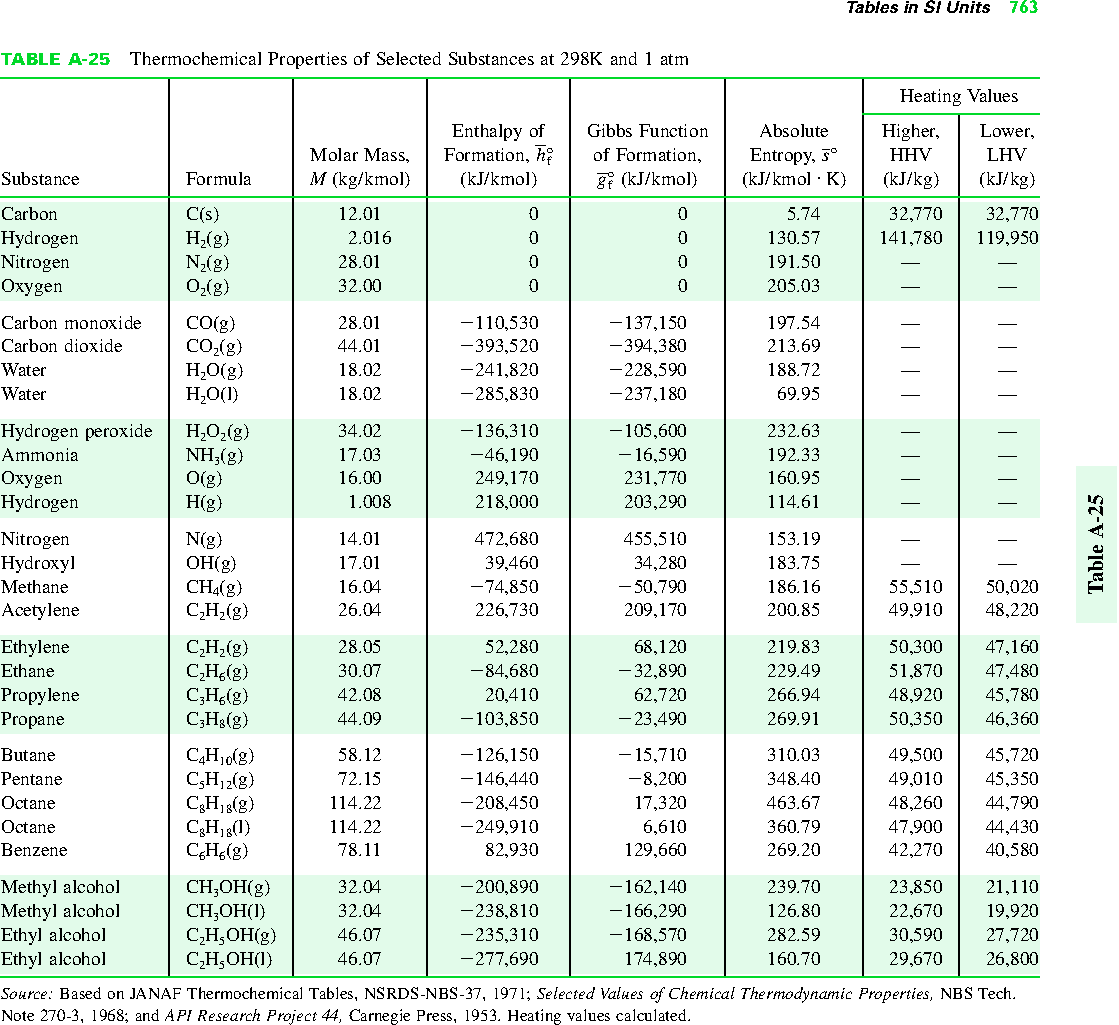
\includegraphics[width=.7\columnwidth,clip]{./../Pics/EnthalpyFormationTable2}
     \end{center} 
\end{frame}
\normalsize



%%%
%%% Slide
%%%
%\scriptsize
\begin{frame}
  \frametitle{Standard Enthalpy of Reaction}
      Given the homogeneous reaction:
        \begin{displaymath}
           \visible<1->{\nu_{a}A(g) + \nu_{b}B(g)  + \cdots \Longleftrightarrow \nu_{c}C(g) + \nu_{d}D(g) + \cdots}
        \end{displaymath}
        \visible<2->{\begin{block}{\begin{center}Definition (Devoe, 2012)\end{center}} 
            ``A \red{standard molar reaction enthalpy $\left(\Delta H_{r}^{\circ}\right)$} is the molar integral enthalpy of formation of species taking place under standard state conditions (each reactant and product at unit activity) at constant temperature.''
        \end{block}}

        \visible<3->{\begin{block}{\begin{center} Standard Molar Enthalpy of Reaction \end{center}}
            In other words, the \red{standard molar enthalpy of reaction, $\Delta H_{r}^{\circ}$} (also called {\it standard heat of reaction}), is the heat produced or consumed during a chemical reaction at constant \blue{$T$} and \blue{\it standard pressure $\left(P^{\circ}\right)$ of 1 atm},
           \begin{displaymath}
                \red{\Delta H_{r}^{\circ} = \summation[\nu_{i}\Delta H_{i,f}^{\circ}]{i=1}{\mathcal{C}}},\;\;\blue{\left(T \text{ is often defined as 25}^{\circ}\text{C}\right)}.
           \end{displaymath}
        \end{block}}
\end{frame}
\normalsize

%%%
%%% Slide
%%%
%\scriptsize
\begin{frame}
  \frametitle{Standard Enthalpy of Reaction}
      

      \begin{block}{\begin{center} Exothermic and Endothermic Reactions \end{center}}
          \visible<1->{Given the \blue{standard enthalpy of reaction},
                         \begin{displaymath}
                             \red{\Delta H_{r}^{\circ} = \summation[\left\{\nu_{i}\Delta H_{i,f}^{\circ}(T)\right\}_{\text{prodt}}]{i=1}{\mathcal{C}} + \summation[\left\{\nu_{i}\Delta H_{i,f}^{\circ}(T)\right\}_{\text{react}}]{i=1}{\mathcal{C}} }
                         \end{displaymath} 
                         with \red{$\left(\nu_{i}>0\right)_{\text{prodt}}$} and \blue{$\left(\nu_{i}<0\right)_{\text{react}}$}.
                      }

            \visible<2->{\red{$\Delta H_{r}^{\circ}$} measures the heat associated with the reaction:
               \begin{displaymath}
                   \Delta H_{r}^{\circ} 
                        \begin{cases}
                             > 0: & \text{Reaction is \red{endothermic}, \ie reaction only occurs if heat is } \\
                                  & \hspace{1cm} \text{added to the system}; \\
                             < 0: & \text{Reaction is \blue{exothermic}, \ie reaction produces heat};
                        \end{cases}
               \end{displaymath}}

        \end{block}
\end{frame}
\normalsize

%%%
%%% Slide
%%%
%\scriptsize
\begin{frame}
  \frametitle{Reaction Enthalpy Change at $P^{\circ}$ and $T\ne 25^{\circ}C$}
     \begin{block}{\begin{center}Determining $\Delta H_{r}^{\circ}(T)$\end{center}} 
      Given the homogeneous reaction:
        \begin{displaymath}
           \visible<1->{\nu_{a}A(g) + \nu_{b}B(g) + \cdots \Longleftrightarrow \nu_{c}C(g) + \nu_{d}D(g) + \cdots}
        \end{displaymath}
        \visible<2->{When a reaction takes place at temperature $T\ne 25^{\circ}$C,
           \begin{displaymath}
             \red{\Delta H_{r}^{\circ} = \summation[\left\{\nu_{i}\Delta H_{i,f}^{\circ}(T)\right\}_{\text{prodt}}]{i=1}{\mathcal{C}} + \summation[\left\{\nu_{i}\Delta H_{i,f}^{\circ}(T)\right\}_{\text{react}}]{i=1}{\mathcal{C}} }
           \end{displaymath} 
           where}
        \visible<3->{\begin{displaymath}
             \blue{\Delta H_{i,f}^{\circ}(T) =  \Delta H_{i,f}^{\circ}(T = 298.15 K) + \int\limits_{298.15 K}^{T} \Delta C_{p,i}dT}\;\;\text{ with }\;\;\Delta C_{p,i} = \nu_{i}C_{p,i}
          \end{displaymath}
          $C_{p}$ is often expressed as a polynomial of $T$ and can be obtained from any ChemEng Handbook.}
        \end{block}
\end{frame}
\normalsize

%%%
%%% Slide
%%%
%\scriptsize
\begin{frame}
  \frametitle{Standard Entropy of Reaction}
      Given the homogeneous reaction:
        \begin{displaymath}
           \visible<1->{\nu_{a}A(g) + \nu_{b}B(g) + \cdots \Longleftrightarrow \nu_{c}C(g) + \nu_{d}D(g) + \cdots} 
        \end{displaymath}

        \visible<2->{\begin{block}{\begin{center} Standard Molar Entropy of Reaction \end{center}}
            The \red{standard molar entropy of reaction, $\Delta S_{r}^{\circ}$} at temperature \blue{T} and \blue{\it standard pressure $\left(P^{\circ}\right)$ of 1 atm} is defined as 
           \begin{displaymath}
             \red{\Delta S_{r}^{\circ} = \summation[\left\{\nu_{i}\Delta S_{i,f}^{\circ}(T)\right\}_{\text{prodt}}]{i=1}{\mathcal{C}} + \summation[\left\{\nu_{i}\Delta S_{i,f}^{\circ}(T)\right\}_{\text{react}}]{i=1}{\mathcal{C}} }
           \end{displaymath} 
           where}
        \visible<3->{\begin{displaymath}
             \blue{\Delta S_{i,f}^{\circ}(T) =  \Delta S_{i,f}^{\circ}(T = 298.15 K) + \int\limits_{298.15 K}^{T} \frc{\Delta C_{p,i}}{T}dT}
          \end{displaymath}
        \end{block}}
\end{frame}
\normalsize

%%%
%%% Slide
%%%
%\scriptsize
\begin{frame}
  \frametitle{Standard Gibbs Free Energy of Reaction}
      \begin{enumerate}[a)]
         \item<1-> From the Fundamental Thermodynamic Relations:
              \visible<1->{\begin{displaymath}
                              dG = dH - TdS
                           \end{displaymath}
              }
         \item<2-> The \red{standard Gibbs free energy of reaction} can be obtained from \underline{either} the fundamental thermodynamic relation \underline{or} from tabulated values of \red{standard Gibbs free energy of formation}
      \end{enumerate}
 

        \visible<3->{\begin{block}{\begin{center} Standard Molar Gibbs Free Energy of Reaction \end{center}}
            The \red{standard molar Gibbs free energy of reaction, $\Delta G_{r}^{\circ}$} at temperature \blue{T} and \blue{\it standard pressure $\left(P^{\circ}\right)$ of 1 atm} is defined as 
           \begin{displaymath}
             \red{\Delta G_{r}^{\circ} = \summation[\left\{\nu_{i}\Delta G_{i,f}^{\circ}(T)\right\}_{\text{prodt}}]{i=1}{\mathcal{C}} + \summation[\left\{\nu_{i}\Delta G_{i,f}^{\circ}(T)\right\}_{\text{react}}]{i=1}{\mathcal{C}} }
           \end{displaymath} 
           where}
        \visible<3->{\begin{displaymath}
             \blue{\Delta G_{i,f}^{\circ}(T) =  \Delta H_{i,f}^{\circ}(T) - T \Delta S_{i,f}^{\circ}(T) }
          \end{displaymath}
        \end{block}}
\end{frame}
\normalsize


%%%
%%% Slide
%%%
%\scriptsize
\begin{frame}
  \frametitle{Standard Gibbs Free Energy of Reaction: Direction of Reaction}
      \begin{enumerate}[a)]
          \item<1-> Given the homogeneous reaction:
               \begin{eqnarray}
                  && \nu_{a}A(g) + \nu_{b}B(g) + \cdots \red{\longrightarrow} \nu_{c}C(g) + \nu_{d}D(g) + \cdots \nonumber \\ 
                  && \nu_{a}A(g) + \nu_{b}B(g) + \cdots \blue{\longleftarrow} \nu_{c}C(g) + \nu_{d}D(g) + \cdots \nonumber
               \end{eqnarray}
               \visible<2->{What is the direction at $T$ and $P$? Towards the products ? Or towards the reactants?}
      \end{enumerate}

        \visible<3->{\begin{block}{\begin{center} Direction of Reaction (\ie Spontaneity) \end{center}}
            The direction of a chemical reaction can be determined based on the \red{standard molar Gibbs free energy of reaction, $\Delta G_{r}^{\circ}$} at temperature \blue{T} and \blue{$\left(P^{\circ}\right)$}:
           \begin{displaymath}
                 \Delta G_{r}^{\circ}(T)
               \begin{cases}
                   < 0: & \text{Reaction towards the formation of products \red{(spontaneous)}}; \\ 
                   = 0: & \text{Reaction is at equilibrium, \ie no further change occurs}; \\ 
                   > 0: & \text{Reaction will not proceed or occur toward the formation of}\\ 
                        & \hspace{1cm} \text{ reactants \blue{(non-spontaneous)}}.
               \end{cases}
           \end{displaymath} 
        \end{block}}
\end{frame}
\normalsize



%%%
%%% SECTION
%%%
\section{Reaction Equilibrium}
\subsection{General Remarks}

%%%
%%% Slide
%%%
%\scriptsize
\begin{frame}
  \frametitle{Reaction Equilibrium: General Remarks}
  \begin{columns}
     \begin{column}[l]{0.5\linewidth}\scriptsize
      \begin{figure}%
        \begin{center}
          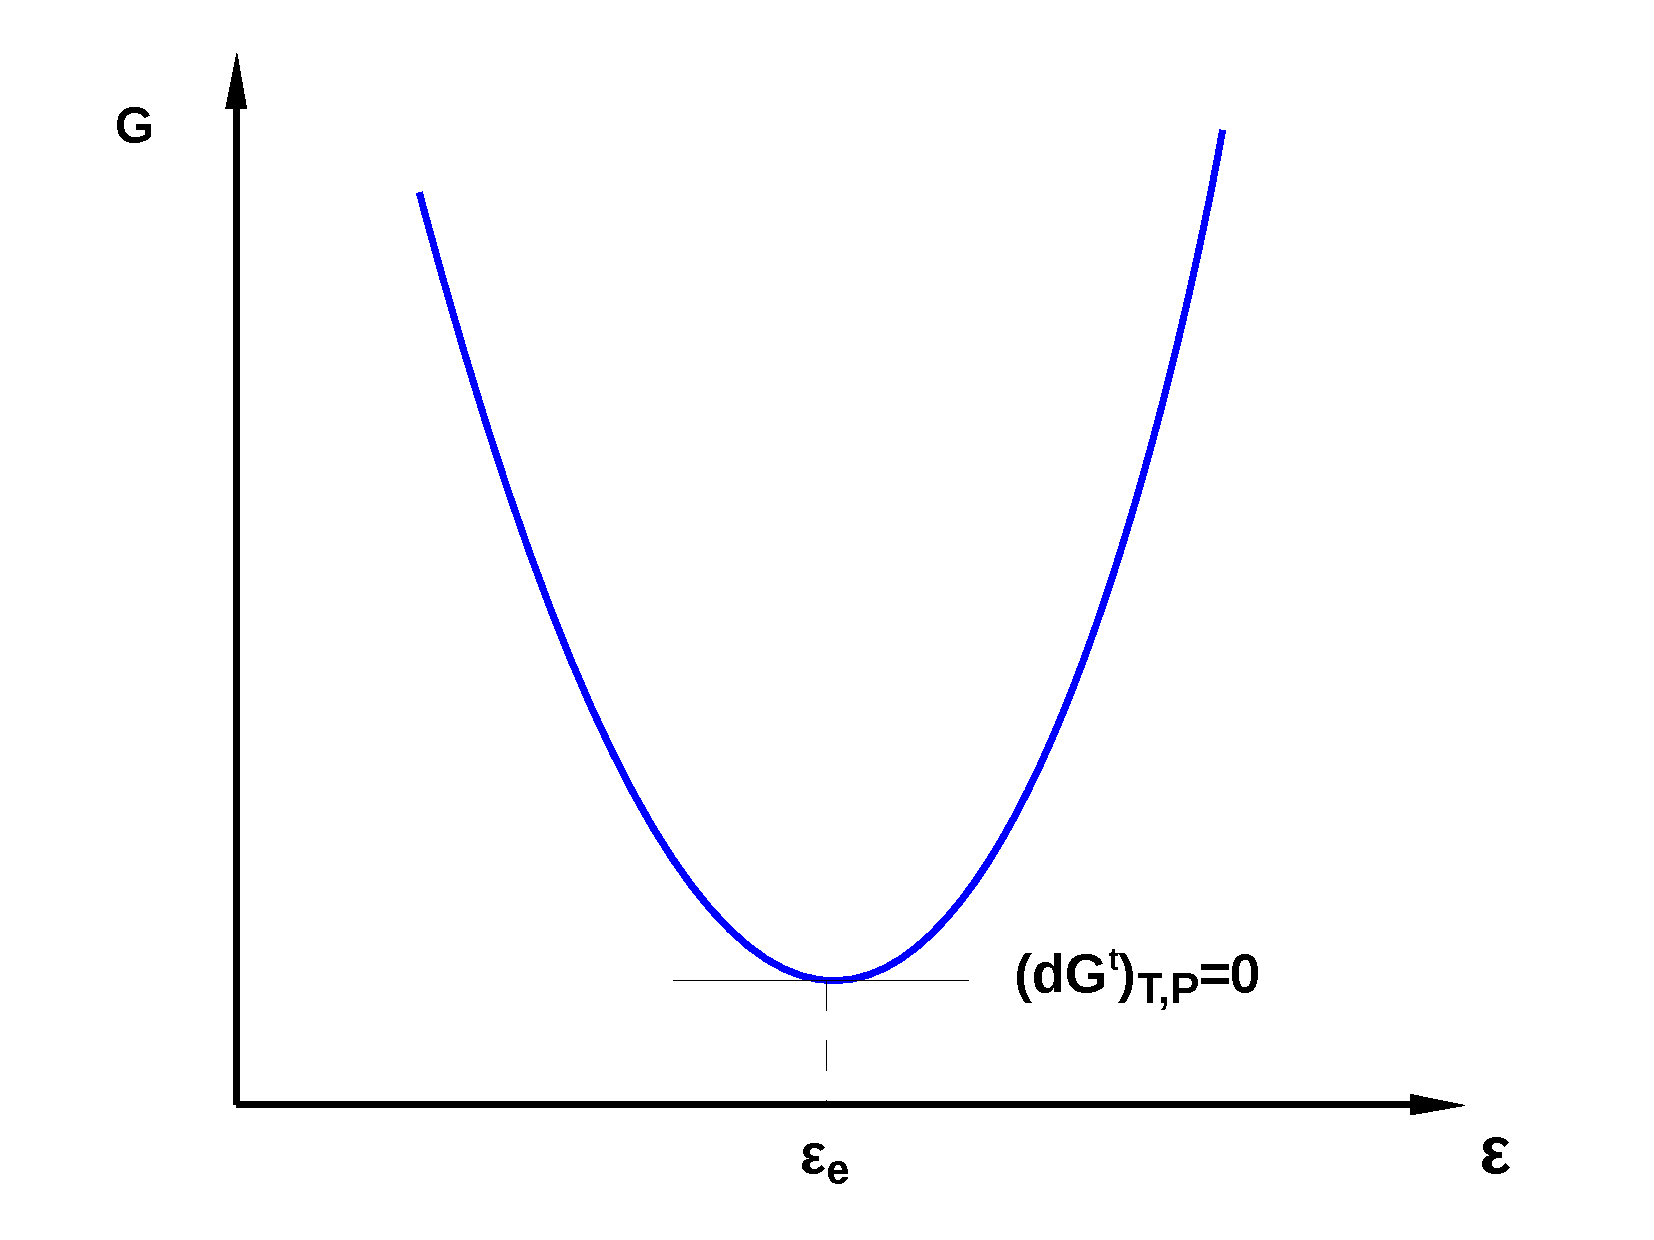
\includegraphics[width=1.05\columnwidth,clip]{./../Pics/ChemicalReactions_GxPlot}
        \end{center}
      \end{figure}
     \end{column}
     \begin{column}[l]{0.5\linewidth}%\scriptsize
        \begin{enumerate}[a)] 
           \item<1-> From \blue{Module 03}, we studied that the equilibrium criteria can be described as function of state properties (i.e., $G$, $S$, $U$, $H$ and $A$);
           \item<2-> In reactive systems, at constant $T$ and $P$, the equilibrium is reached when the \blue{total Gibbs energy} is \red{minimum}, i.e., 
               \visible<2->{\begin{displaymath}
                  \left(\frc{d G^{t}}{d\varepsilon}\right)_{T,P} = 0 
               \end{displaymath}}
        \end{enumerate}
     \end{column}
  \end{columns}
\end{frame}
\normalsize


%%%
%%% SUBSECTION
%%%
\subsection{Equilibrium Constant}

%%%
%%% Slide
%%%
%\scriptsize
\begin{frame}
  \frametitle{Reaction Equilibrium: Equilibrium Constant}
      \begin{enumerate}[a)]
         \item<1-> The \red{equilibrium} of a chemical reaction is reached when \blue{$\Delta G_{r}^{\circ}(T)=0$},
         \item<2-> For example, given the homogeneous reactions:
              \visible<2->{
             \reaction{ NH_{3} (aq) + H_{2}O (l) <=> NH_{4}^{+} (l) + OH^{-} (aq) }
             At equilibrium (with constant $T$ and $P$),
                \begin{displaymath}
                    \underbrace{\frc{\left[NH_{4}^{+}\right].\left[OH^{-}\right]}{\left[NH_{3}\right].\left[H_{2}O\right]}}_{\text{reaction quotient}} = \text{constant},
                \end{displaymath}
             where \blue{[]} represents either concentration or activity of species.}
            \visible<3->{And,
             \reaction{ 2 NO (g) + O_{2} (g) <=> 2 NO_{2} (g) }
             At equilibrium (with constant $T$ and $P$),
                \begin{displaymath}
                    \underbrace{\frc{P_{\text{NO}_{2}}^{2}}{P_{\text{NO}}^{2}.P_{\text{O}_{2}}}}_{\text{reaction quotient}} = \text{constant},
                \end{displaymath}}
            \visible<4->{At \blue{equilibrium the reaction quotient} \red{(K)} \blue{becomes \underline{constant}.}}
      \end{enumerate}
\end{frame}


%%%
%%% Slide
%%%
%\scriptsize
\begin{frame}
  \frametitle{Reaction Equilibrium: Equilibrium Constant}
        \begin{displaymath}
           \visible<1->{\nu_{a}A + \nu_{b}B  \Longleftrightarrow \nu_{c}C + \nu_{d}D } 
        \end{displaymath}
      \begin{enumerate}[a)]\setcounter{enumi}{2}
         \item<1-> The \blue{equilibrium} is a state in which no further change is possible under specific parameters, \ie 
         \item<1-> The rate of the forward reaction is equal to the reverse reaction;
         \item<2-> Any changes of the reaction parameters (\eg addition of chemical species, changes in pressure and/or temperature conditions) may lead to new equilibrium, which may not be the same as the previous one;
         \item<3-> The \blue{reaction quotient}, \red{K}, is called \red{\it equilibrium constant} and establishes a relationship between activities (or concentration for ideal systems or partial pressures for gas mixtures) of species in equilibrium;
         \item<3-> \red{$K$} does not give any information on {\it how fast a reaction proceeds}. This is controlled by \blue{reaction kinetics} which is not the focus of our study.
      \end{enumerate}
\end{frame}


%%%
%%% Slide
%%%
%\scriptsize
\begin{frame}
  \frametitle{Reaction Equilibrium: Equilibrium Constant}
      \begin{enumerate}[a)]\setcounter{enumi}{7}
        \item<1-> The total Gibbs free energy of homogeneous chemical reactions can be represented by the individual contributions of reacting species,
            \visible<1->{\begin{displaymath}
                G^{t} = \summation[n_{i}\overline{G}_{i}]{i=1}{\mathcal{C}} = \summation[\left(n_{i,0}+\nu_{i}\varepsilon\right)\overline{G}_{i}]{i=1}{\mathcal{C}},
            \end{displaymath}
            where $\overline{G}_{i}$ is the partial molar Gibbs energy of component $i$}.
      \end{enumerate}

      \begin{block} {\begin{center}Equilibrium Criteria\end{center}}
            \visible<2->{\begin{displaymath}
                \summation[\nu_{i}\overline{G}_{i}]{i=1}{\mathcal{C}} = 0  = \summation[\nu_{i}\mu_{i}]{i=1}{\mathcal{C}}, 
            \end{displaymath}}
          \visible<3->{where {\it standard state} \blue{$\left(^{\circ}\right)$} is the state in which}
                  \begin{enumerate}[i)]
                      \item<3-> $P=1$ atm {\bf and};
                      \item<3-> Component is pure $\left(\text{\ie } x_{i}^{\circ}=1\right)$ {\bf or } component at infinite dilution $\left(\text{\ie } x_{i}^{\infty}=x_{i}^{\circ}=0\right)$ {\bf or} {\it ideal 1 molal solution}.
                   \end{enumerate}
      \end{block}

\end{frame}

%%%
%%% Slide
%%%
%\scriptsize
\begin{frame}
  \frametitle{Reaction Equilibrium: Equilibrium Constant}
      \begin{enumerate}[a)]\setcounter{enumi}{8}
        \item<1-> Thus the difference between states
            \begin{center}
                 \blue{(Gibbs at reaction conditions - Gibbs at standard conditions)},
            \end{center}
            can be represented by {\it activities} of the reacting species, \ie
            \visible<2->{\begin{displaymath}
                \overline{G}\left(T,P, x_{i}\right)  - \overline{G}_{i}^{\circ}\left(T,P=1\text{ atm}, x_{i}^{\circ}\right) = RT\ln{\frc{\overline{f}_{i}}{\overline{f}_{i}^{\circ}}} = RT\ln{a_{i}},
            \end{displaymath}}
            \visible<2->{where
            \begin{displaymath}
               \begin{cases}
                    \overline{f}_{i}: & \text{fugacity of component } i \text{ in the mixture}; \\
                    \overline{f}_{i}^{\circ}: & \text{fugacity of component } i \text{ in the mixture at standard conditions}; \\
                    a_{i}: & \text{activity of component } i \text{ in the mixture}.
               \end{cases}
            \end{displaymath}}
      \end{enumerate}
\end{frame}



%%%
%%% Slide
%%%
%\scriptsize
\begin{frame}
  \frametitle{Reaction Equilibrium: Equilibrium Constant}
      \begin{block}{\begin{center}Equilibrium Constant\end{center}}
            Let's consider the generic chemical reaction,
               \begin{displaymath}
                   \nu_{1} A_{1} + \nu_{2} A_{2}  + \cdots  \Longleftrightarrow \nu_{m} A_{m} + \nu_{n} A_{n} + \cdots  
               \end{displaymath} 
            The equilibrium constant $K$ is expressed as,
               \begin{displaymath}
                  \blue{K = \exp\left(\frc{-\Delta G_{r}^{\circ}}{RT}\right) = \prod\limits_{i=1}^{\mathcal{C}}\left(\frc{\overline{f}_{i}}{\overline{f}_{i}^{\circ}}\right)^{\nu_{i}} = \prod\limits_{i=1}^{\mathcal{C}} a_{i}^{\nu_{i}}}
               \end{displaymath}
               where $\Delta G_{r}^{\circ}=\summation[\nu_{i}\overline{G}_{i}^{\circ}\left(T,P=1\text{ atm}, x_{i}^{\circ}\right)]{i}{}$ is the Gibbs energy change on reaction with each species (reactants and products) in its standard state.
      \end{block}

\end{frame}



%%%
%%% Slide
%%%
%\scriptsize
\begin{frame}
  \frametitle{Reaction Equilibrium: Equilibrium Constant}
       \begin{block}{\begin{center}Equilibrium Constant\end{center}}
            Let's consider a chemical reaction in {\it equilibrium},
               \begin{displaymath}
                   \nu_{a} A + \nu_{b} B \Longleftrightarrow \nu_{c} C + \nu_{d} D 
               \end{displaymath} 
          \begin{center}
            \begin{tabular}{l | c c}
               \hline
                  {\bf Ideal Gas} & $\Delta G_{r}^{\circ}=-RT\ln{K_{p}}=\Delta\mu_{r}^{\circ}$ & $K_{p} = \frc{P_{C}^{c}.P_{D}^{d}}{P_{A}^{a}.P_{B}^{b}}$ \\
                                  &                                                &                                                         \\
                  {\bf Real Gas}  & $\Delta \mu_{r}^{\circ}=-RT\ln{K_{f}}$               &  $K_{f} = \frc{f_{C}^{c}.f_{D}^{d}}{f_{A}^{a}.f_{B}^{b}} K_{p}$ \\
                                  &                                                &                                                         \\
                  {\bf Ideal Solution} & $\Delta G_{r}^{\circ}=-RT\ln{K_{c}}=\Delta\mu_{r}^{\circ}$ & $K_{c} = \frc{[C]^{c}.[D]^{d}}{[A]^{a}.[B]^{b}}$ \\
                                  &                                                &                                                         \\
                  {\bf Real Solution} & $\Delta\mu_{r}^{\circ}=-RT\ln{K_{a}}$             &  $K_{a} = \frc{a_{C}^{c}.a_{D}^{d}}{a_{A}^{a}.a_{B}^{b}} K_{c}$\\
                                  &                                                &                                                         \\
               \hline
            \end{tabular}
           \end{center}
 
       \end{block}
\end{frame}

%%%
%%% Slide
%%%
%\scriptsize
\begin{frame}
  \frametitle{Reaction Equilibrium:  Dependence of $K$ with Temperature } 
     \begin{center}
          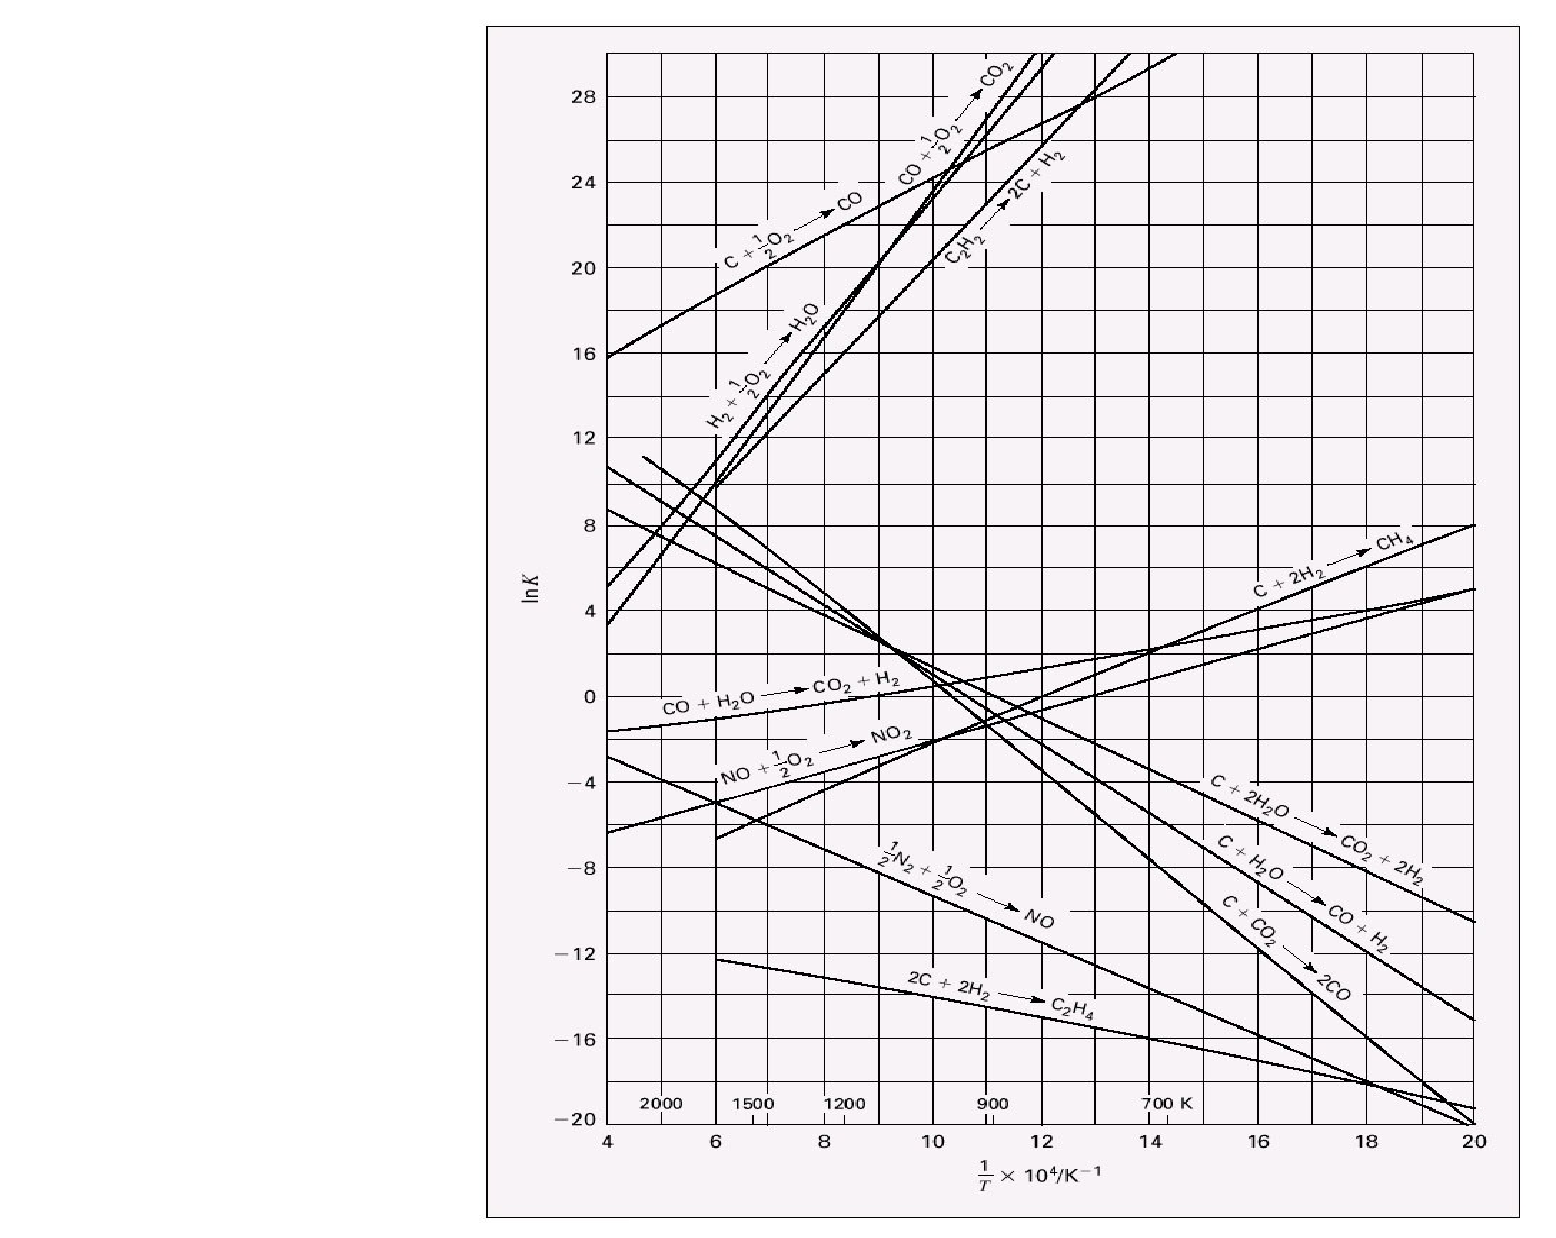
\includegraphics[width=.95\columnwidth,height=0.65\columnwidth,clip]{./../Pics/ChemicalReactions_EquilConstPlotb} 
     \end{center} 

\end{frame}
%%%
%%% Slide
%%%
%\scriptsize
\begin{frame}
  \frametitle{Reaction Equilibrium:  Dependence of $K$ with Temperature } 


      \visible<1->{\begin{block}{\begin{center}Van't Hoff Equation\end{center}}
            The \blue{Van't Hoff equation} can help obtaining the {\it equilibrium constant} \red{at any temperature by integrating from $T=298.15$ K} to \red{T},
               \begin{displaymath}
                 \frc{d\left(\ln{K}\right)}{dT} = \frc{\Delta H^{\circ}_{r}}{RT^{2}} \;\;\;\;\;\text{ or }\;\;\;\;\; \frc{d}{dT}\left(\Delta G^{\circ}_{r}/RT\right) = -\frc{d\left(\ln{K}\right)}{dT} = -\frc{\Delta H^{\circ}_{r}}{RT^{2}}
               \end{displaymath} 
            where $\Delta H^{\circ}_{r}$ is the {\it standard heat (or enthalpy) of reaction}.
      \end{block}}
\end{frame}

%%%
%%% Slide
%%%
%\scriptsize
\begin{frame}
  \frametitle{Reaction Equilibrium:  Dependence of $K$ with Composition } 
      \begin{enumerate}[a)] \setcounter{enumi}{9} 
         \item<1-> From 
           \begin{displaymath}
                K = \prod\limits_{i=1}^{\mathcal{C}} a_{i}^{\nu_{i}} = \prod\limits_{i=1}^{\mathcal{C}} \left(\frc{\overline{f}_{i}}{\overline{f}_{i}^{\circ}}\right)^{\nu_{i}},
           \end{displaymath} 
         \item<2-> And considering for gaseous species that $\overline{f}_{i}^{\circ}=P^{\circ}=1$ atm and $\overline{f}_{i} = \overline{\phi}_{i}y_{i}P$;
      \end{enumerate}

      \visible<3->{\begin{block}{\begin{center}Gaseous Phase\end{center}}
               \begin{eqnarray}
                  && \prod\limits_{i=1}^{\mathcal{C}} \left(\overline{\phi}_{i}y_{i}\right)^{\nu_{i}} = K\left(\frc{P}{P^{\circ}}\right)^{-\nu}\;\;\;\;\blue{\text{ (for gaseous phase).}} \nonumber\\
                  && \prod\limits_{i=1}^{\mathcal{C}} y_{i}^{\nu_{i}} = K\left(\frc{P}{P^{\circ}}\right)^{-\nu}\;\;\;\;\blue{\text{ (for ideal gases).}}\nonumber
               \end{eqnarray} 
      \end{block}
      where $\nu=\summation[\nu_{i}]{i}{}$,}
\end{frame}
%%% Slide
%%%
%\scriptsize
\begin{frame}
  \frametitle{Reaction Equilibrium:  Dependence of $K$ with Composition } 
      \begin{enumerate}[a)] \setcounter{enumi}{11} 
         \item<1-> From 
           \begin{displaymath}
                K = \prod\limits_{i=1}^{\mathcal{C}} a_{i}^{\nu_{i}} = \prod\limits_{i=1}^{\mathcal{C}} \left(\frc{\overline{f}_{i}}{\overline{f}_{i}^{\circ}}\right)^{\nu_{i}},
           \end{displaymath} 
         \item<2-> And using $\overline{f}_{i} = \gamma_{i}x_{i}f_{i}$, where $f_{i}$ is the fugacity of pure component $i$ in the liquid phase at $P$ and $T$
      \end{enumerate}

      \visible<3->{\begin{block}{\begin{center}Liquid Phase\end{center}}
               \begin{displaymath}
                     \prod\limits_{i=1}^{\mathcal{C}}\left(\gamma_{i}x_{i}\right)^{\nu_{i}} = K\exp{\left[\frc{P^{\circ}-P}{RT}\summation[V_{i}\nu_{i}]{i=1}{\mathcal{C}}\right]}\;\;\;\;\blue{\text{ (for liquid phase).}}
               \end{displaymath} 
           and for the following particular cases,
               \begin{displaymath}
                      K = 
                          \begin{cases}
                               \prod\limits_{i=1}^{\mathcal{C}}\left(\gamma_{i}x_{i}\right)^{\nu_{i}}  & \blue{\text{ (for liquid phase at room pressure conditions);}}  \\
                               \prod\limits_{i=1}^{\mathcal{C}}x_{i}^{\nu_{i}}  & \blue{\text{ (for ideal solutions).}} 
                          \end{cases}
               \end{displaymath}
      \end{block}}
\end{frame}

%%%
%%% SUBSECTION
%%%
%\subsection{Phase Rule}

%%%
%%% Slide
%%%
%\scriptsize
%\begin{frame}
%  \frametitle{Reaction Equilibrium: Phase Rule}
%     \begin{enumerate}[a)] %\setcounter{enumi}{4}
%        \item<1-> Recall the Gibbs phase rule (Module 1) for \blue{non-reacting multiphase and multi-component systems}:
%           \visible<1->{\begin{displaymath}
%             \Psi = 2 + \mathcal{C} - \mathcal{P}
%           \end{displaymath}
%             where $\Psi$ is the number of \textcolor{blue}{degrees of freedom} for the system, \textcolor{blue}{2} refers to the independent variables ($T$ and $P$), \textcolor{blue}{$\mathcal{C}$} is the number of chemical species and \textcolor{blue}{$\mathcal{P}$} is the number of phases;}   
%        \item<2->For a multiphase, multi-component systems with \red{$\mathcal{R}$ chemical reactions} take place: 
%           \visible<1->{\begin{displaymath}
%              \blue{\Psi = 2 + \mathcal{C} - \mathcal{P} - \mathcal{R}}
%           \end{displaymath}}
%     \end{enumerate}
%\end{frame}
%\normalsize

%%%
%%% SUBSECTION
%%%
\subsection{Multi-Reaction Equilibrium}

%%% Slide
%%%
%\scriptsize
\begin{frame}
  \frametitle{Multiple Simultaneous Reactions}
      Let's consider a set of $\mathcal{R}$ {\it independent reactions} involving $\mathcal{C}$ chemical species, 
               \begin{eqnarray}
                     \nu_{1,1}A_{1,1} (g) + \nu_{2,1}A_{2,1} &\Longleftrightarrow& \nu_{3,1}A_{3,1} (g) + \nu_{4,1}A_{4,1} (g) \nonumber\\
                     \nu_{5,2}A_{5,2} (g) + \nu_{6,2}A_{6,2} &\Longleftrightarrow& \nu_{7,2}A_{7,2} (g) + \nu_{8,2}A_{8,2} (g)  \nonumber\\
                                 \vdots               &\Longleftrightarrow&     \vdots                         \nonumber\\
                     \nu_{\mathcal{C}-3,\mathcal{R}}A_{\mathcal{C}-3,\mathcal{R}} (g) + \nu_{\mathcal{C}-2,\mathcal{R}}A_{\mathcal{C}-2,\mathcal{R}} &\Longleftrightarrow& \nu_{\mathcal{C}-1,\mathcal{R}}A_{\mathcal{C}-1,\mathcal{R}} (g) + \nu_{\mathcal{C},\mathcal{R}}A_{\mathcal{C},\mathcal{R}} (g) \nonumber
               \end{eqnarray}
      the equilibrium constant for each reaction is given by an extension of the previous equations

        \visible<1->{\begin{block}{\begin{center}Simultaneous Reactions\end{center}}
               \begin{displaymath}
                      K_{j} = 
                          \begin{cases}
                               \prod\limits_{i=1}^{\mathcal{C}} \left(\frc{\overline{f}_{i}}{P^{\circ}}\right)^{\nu_{i,j}}, & \blue{\text{(gas phase),}} \\
                                                                   & \\
                               \left(\frc{P}{P^{\circ}}\right)^{-\nu_{i,j}}\prod\limits_{i=1}^{\mathcal{C}} \left(y_{i}\right)^{\nu_{i,j}}, &\blue{\text{(ideal gas mixture).}}
                          \end{cases}\hspace{1cm} \forall j\in\left\{1,2,\cdots,\mathcal{R}\right\}
               \end{displaymath}
      \end{block}}

\end{frame}
\normalsize

\section{Summary}

%%%
%%% Slide
%%%
%\scriptsize
\begin{frame}
 \frametitle{Summary}
   After this Module, you should be able to:
   \begin{enumerate}[(i)]
     \item Identify and make use of chemical notation for reacting thermodynamic systems;
     \item Identify thermodynamic criteria for chemical equilibrium;
     \item Make use of equilibrium constant definition and its dependence on system parameters;
     \item Apply phase rule for reacting systems.
   \end{enumerate}
\end{frame}

\begin{comment}
\section{Examples}

%%%
%%% Slide
%%%
%\scriptsize
\begin{frame}
 \frametitle{Example 1:}
     \blue{Calculate the equilibrium extent of decomposition of nitrogen tetroxide $\left(N_{2}O_{4}\right)$,}
        \begin{displaymath}
           \blue{N_{2}O_{4} (g) \Longleftrightarrow 2 NO_{2} (g)}
        \end{displaymath}
        \blue{at 25$^{\circ}$C and 1 atm. Assume that the gas mixture behaves as an ideal gas and the Gibbs energies of formation at 25$^{\circ}$C are:}
        \begin{displaymath}
          \blue{ \left(\Delta G^{\circ}_{\text{f,298}}\right)_{N_{2}O_{4}} = 97.89 \text{ kJ.mol}^{-1} \text{ and } \left(\Delta G^{\circ}_{\text{f,298}}\right)_{NO_{2}} = 51.31 \text{ kJ.mol}^{-1}.}
        \end{displaymath}
     
\end{frame}

%%%
%%% Slide
%%%
%\scriptsize
\begin{frame}
 \frametitle{Example 2:}
     \blue{Ethylene is produced from the decomposition of ethane,}
       \begin{displaymath}
          \blue{C_{2}H_{6} (g) \Longleftrightarrow C_{2}H_{4} (g) + H_{2} (g) }
       \end{displaymath} 
       \blue{Determine the equilibrium composition at 1000$^{\circ}$C and 1 atm. Assume that, initially, there is 1 mol of ethane. Given,}
       \begin{center}
           \blue{\begin{tabular}{|c c c c|}
           \hline
                                        &  C$_{2}$H$_{6}$ (g) & C$_{2}$H$_{4}$ (g) &  H$_{2}$ (g)  \\ 
           \hline
             $\Delta G^{\circ}_{\text{f,298}}$  &  -32.84            &  68.15           & 0.0           \\
                   (kJ/mol)             &                    &                  &               \\
           \hline
             $\Delta H^{\circ}_{\text{f,298}}$  &  -84.68            &  52.26           & 0.0           \\
                   (kJ/mol)             &                    &                  &               \\
           \hline 
           \end{tabular}}
       \end{center}
       \blue{where $\Delta G^{\circ}_{\text{f,298}}$ and $\Delta H^{\circ}_{\text{f,298}}$ are the standard state Gibbs energy and enthalpy of formation. }
     
\end{frame}
\end{comment}

\end{document}
 
